\subsection{Small-Budget Estimation of Consumer Disagreement}\label{app:query_risk}

The finite-corpus check answers whether a candidate meets a disagreement
budget. A small sample can also estimate the amount of disagreement, although
direct binary counts have substantial sampling variation. We test whether
statistical propagation through the cheap reader improves this estimate.
Conditional-expectation variance reduction and model-assisted estimation are
established tools; prediction-powered inference~\citep{angelopoulos2023ppi}
provides related context for combining inexpensive predictions with exact samples.
Here we evaluate point-estimation error, separately from the earlier certificate.

Let $Z$ be repaired current logits and $E$ the healthy-minus-current logit
residual. A known conditional law gives
$m_j(Z)=\Pr\{C_j(Z+E)\ne C_j(Z)\mid Z\}$ for consumer $j$.
Then $\mathbb E m_j(Z)=\Pr\{C_j(Z+E)\ne C_j(Z)\}$ and the conditional-variance
identity gives $\operatorname{Var}(m_j(Z))\le\operatorname{Var}(\mathbf1\{C_j(Z+E)\ne C_j(Z)\})$.
We approximate the residual law by a shared Gaussian mean/covariance estimated
from a small monitor, with $10\%$ shrinkage toward an isotropic covariance.
An isotropic comparator retains the same mean and covariance trace.

An exploratory screen on all six earlier visual development endpoints fixes the
recipe before confirmation. Each repair uses $1{,}024$ isolated anchors to fit
a standardized centered-logit ridge reader with coefficient $10^{-3}$.
A separate $1{,}024$-anchor pool supplies monitor subsets of size $32/64/128/256$.
Both estimators use the same subsets. Propagation averages $64$ fixed Gaussian
draws over $512$ inexpensive current outputs; direct counting uses the observed
old/current consumer differences. No consumer labels enter either estimator.
The additional monitor-query budget is separate from the initial $1{,}024$
paired map-fitting outputs, which can be cached across updates.

Confirmation uses the twelve saved CE-only ViT endpoints from four independently
fitted references and partitions, with three continuation seeds per reference.
Their training accuracies were previously observed, but the new repair and risk
outcomes were computed after freezing this analysis. The primary target is the
maximum class/selective disagreement over $5{,}000$ clean validation inputs.
Twenty monitor subsets measure each endpoint's sampling variation. Intervals
use four reference means, each averaging three continuations and their subsets
($t$, three degrees of freedom). The official test split remains closed.

At $32$ additional queries, covariance propagation reduces MAE from $4.773$ to
$0.509$ points; the paired reduction is $4.264$ points, $95\%$ interval
$[3.148,5.380]$. At $64$ queries, MAE falls from $2.964$ to $0.502$, a reduction
of $2.462$ points $[1.573,3.352]$. Both pass the fixed $20\%$ improvement and
positive-lower-interval criteria. With augmented validation inputs and clean
monitor anchors, the corresponding MAEs are $0.690/0.683$ against
$4.228/2.434$, with positive improvement intervals at both primary budgets.
The augmented-view intervals cross zero at $128/256$ queries.

\begin{figure}[H]
\centering
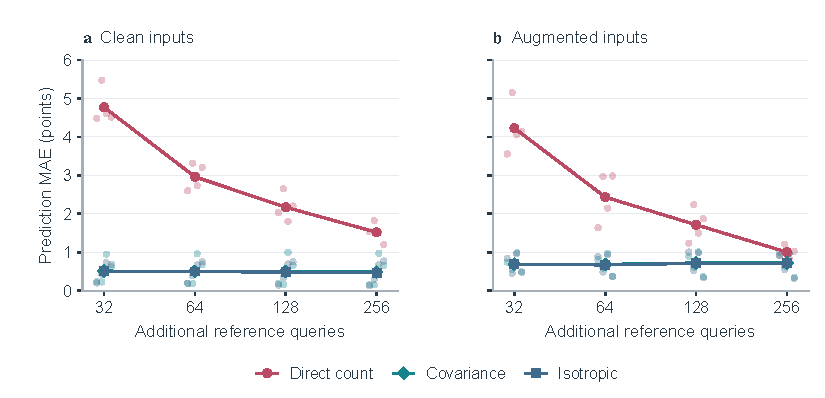
\includegraphics[width=\linewidth]{figures/fig_risk_queries.pdf}
\caption{Reference-query budget and disagreement-estimation error.
Solid markers average four fitted references; pale points show every reference
mean, each averaging three continuations and twenty monitor subsets. Budgets
count additional reference calls after the common $1{,}024$ map-fitting anchors.
The two propagation models additionally use $512$ cheap current outputs.
(a) Clean validation. (b) Fixed augmented views with clean monitor anchors.
The isotropic control ties full covariance within uncertainty.}
\label{fig:query_risk}
\end{figure}

The isotropic model obtains $0.508/0.499$ points at $32/64$ queries; its difference
from full covariance is unresolved. Thus covariance directions add no established
benefit here. Independent rate-level replay reproduces all forecasts. Averaging
absolute errors across the three consumers instead of taking their maximum
retains the gain: clean $32/64$ MAEs are $0.772/0.779$ versus $3.488/2.514$ for
direct counting. The result is not solely a maximum-of-counts effect.

The Gaussian law is an approximation. Marginal residual moments alone cannot
identify disagreement: binary logits $Z=\pm a$ with equal probability and
$E=2Z$ or $E=-2Z$ have identical marginal laws for $Z,E$, yet zero or complete
sign disagreement. Their dependence differs. The estimator therefore supplies
no distribution-free safety certificate. Actual confirmation disagreements are
$6.20$--$7.96\%$, above the $1\%$ repair limit: accurately estimating failure does
not repair it. Query reductions also do not establish end-to-end runtime savings.
The raw output arrays, fixed plans and independent replay are included separately
from raw images and pretrained weights.
